\documentclass[14pt, a4paper]{extarticle}
\usepackage{GOST}
\usepackage{array}
\usepackage{verbatim}
\usepackage[detect-all]{siunitx}
\usepackage{amsmath}
\usepackage{amssymb}
\usepackage[utf8]{inputenc}
\usepackage{hyperref}

\usepackage{ifthen}


\usepackage{tempora}


\makeatletter
\renewcommand\@biblabel[1]{#1.}
\makeatother

% Для листинга кода:
\usepackage{listings}
\lstset{ %
	language=python,                 % выбор языка для подсветки (здесь это С)
	basicstyle=\small\sffamily, % размер и начертание шрифта для подсветки кода
	numbers=left,               % где поставить нумерацию строк (слева\справа)
	numberstyle=\tiny,           % размер шрифта для номеров строк
	stepnumber=1,                   % размер шага между двумя номерами строк
	numbersep=5pt,                % как далеко отстоят номера строк от подсвечиваемого кода
	showspaces=false,            % показывать или нет пробелы специальными отступами
	showstringspaces=false,      % показывать или нет пробелы в строках
	showtabs=false,             % показывать или нет табуляцию в строках
	frame=single,              % рисовать рамку вокруг кода
	tabsize=2,                 % размер табуляции по умолчанию равен 2 пробелам
	captionpos=t,              % позиция заголовка вверху [t] или внизу [b] 
	breaklines=true,           % автоматически переносить строки (да\нет)
	breakatwhitespace=false, % переносить строки только если есть пробел
	escapeinside={\#*}{*)}   % если нужно добавить комментарии в коде
}


%для графиков
\usepackage{pgfplots}
\usepackage{filecontents}
\usetikzlibrary{datavisualization}
\usetikzlibrary{datavisualization.formats.functions}

\begin{document}
	
	\begin{table}[ht]
		\centering
		\begin{tabular}{|c|p{400pt}|} 
			\hline
			\begin{tabular}[c]{@{}c@{}} 
\includegraphics[scale=1]{baum.jpg} \\\end{tabular} &
			\footnotesize\begin{tabular}[c]{@{}c@{}}\textbf{Министерство~науки~и~высшего~образования~Российской~Федерации}\\\textbf{Федеральное~государственное~бюджетное~образовательное~учреждение}\\\textbf{~высшего~образования}\\\textbf{«Московский~государственный~технический~университет}\\\textbf{имени~Н.Э.~Баумана}\\\textbf{(национальный~исследовательский~университет)»}\\\textbf{(МГТУ~им.~Н.Э.~Баумана)}\\\end{tabular}  \\
			\hline
		\end{tabular}
	\end{table}
	\noindent\rule{\textwidth}{4pt}
	\noindent\rule[14pt]{\textwidth}{1pt}
	\hfill 
	\noindent
	\makebox{ФАКУЛЬТЕТ~}%
	\makebox[\textwidth][l]{\underline{~«Информатика и системы управления»~~~~~~~~~~~~~~~~~~~~~~~~~~~~~~~~~}}%
	\\
	\noindent
	\makebox{КАФЕДРА~}%
	\makebox[\textwidth][l]{\underline{~«Программное обеспечение ЭВМ и информационные технологии»~}}%
	
	
	\begin{center}
		\vspace{1.5cm}
		{\bf\huge Отчёт\par}
		{\bf\Large по лабораторной работе № 6\par}
		\vspace{0.7cm}
	\end{center}
	
	
	\noindent
	\makebox{\large{\bf Название:}~~~}
	\makebox[\textwidth][l]{\large\underline{Моделирование парка аттракционов~~~~~~}}
	
	\noindent
	\makebox{\large{\bf Дисциплина:}~~~}
	\makebox[\textwidth][l]{\large\underline{~Моделирование~~~~~~~~~~~~~~~~~~~~~~~~~~}}\\
	
	\vspace{1.5cm}
	\noindent
	\begin{tabular}{l c c c c c}
		Студент      & ~ИУ7-75Б~               & \hspace{2.5cm} & \hspace{2cm}                 & &  Д.В. 
		Сусликов \\\cline{2-2}\cline{4-4} \cline{6-6} 
		\hspace{3cm} & {\footnotesize(Группа)} &                & {\footnotesize(Подпись, дата)} & & {\footnotesize(И.О. Фамилия)}
	\end{tabular}
	
	\noindent
	\begin{tabular}{l c c c c}
		Преподаватель & \hspace{5cm}   & \hspace{2cm}                 & & ~~~~~~И.В. Рудаков~~~~~~\\\cline{3-3} \cline{5-5} 
		\hspace{3cm}  &                & {\footnotesize(Подпись, дата)} & & {\footnotesize(И.О. Фамилия)}
	\end{tabular}
	
	\vspace{0.6cm}
	\begin{center}	
		\vfill
		\large \textit {Москва, 2021}
	\end{center}
	
	\thispagestyle {empty}
	\pagebreak
	
	% СОДЕРЖАНИЕ 
	\clearpage
	\tableofcontents
		
	% ВВЕДЕНИЕ
	\clearpage
	\section*{Задание}
	\addcontentsline{toc}{section}{Задание}
	Реализовать программу для моделирования следующей системы: люди подходят к кассам парка аттракционов с заданным интервалом времени - 1-5. У каждой кассы формируется своя очередь. Посетитель выбирает очередь с минимальной длинной. Кассиры обслуживают клиентов за заданный интервал времени. После того, как посетитель купил билет, он идёт к аттракционам. У каждого аттракциона формируется своя очередь. Посетитель выбирает аттракцион с очередью наименьшей длины. У аттракционов посетителей обслуживают за фиксированный интервал времени. Также посетитель может испугаться аттракциона с вероятностью 25\% и вернуть купленный билет. Количество посетителей задается.\par
	Производительность кассиров:
	\begin{itemize}
		\item Кассир №1 - 2-5;
		\item Кассир №2 - 4-8;
		\item Кассир №1 - 10-15.
	\end{itemize}\par

	Производительность аттракционов:
	\begin{itemize}
		\item Аттракционов №1 - 5-9;
		\item Аттракционов №2 - 10-25.
	\end{itemize}\par
	
	\newpage
	Ниже на Рисунке 1 структурная схема парка аттракционов. 
	\begin{figure}[h!]
		\centering{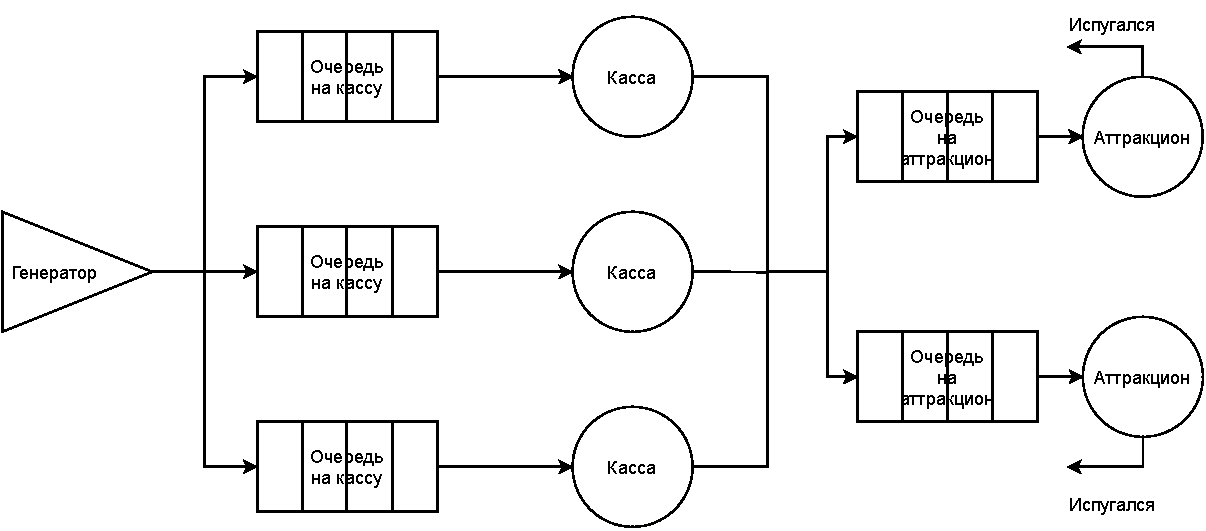
\includegraphics[scale=0.8]{source/scheme.pdf}}
		\centering\caption{Структурная схема}
	\end{figure}
	
	\clearpage
	\section*{Аналитическая часть}
	\addcontentsline{toc}{section}{Аналитическая часть}
	В процессе взаимодействия посетителей с аттракционами возможно:
	
	1) Режим нормального обслуживания, т.е. посетитель посещает понравившийся ему аттракцион.
	
	2) Режим отказа от обслуживания, когда посетитель испугался аттракциона и решил вернуть билет.\par
	
	Формула расчёта вероятности отказа:
	\begin{equation*}
		P_{\text{отк}} = \frac{C_{\text{отк}}}{C_{\text{отк}} + C_{\text{обсл}}}
	\end{equation*}
	
	\clearpage
	\section*{Примеры}
	\addcontentsline{toc}{section}{Примеры}
	
	\begin{figure}[h!]
		\centering{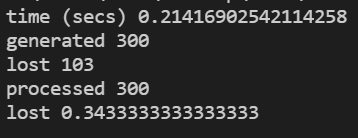
\includegraphics[scale=0.9]{source/1}}
		\centering\caption{300 заявок}
	\end{figure}


	\begin{figure}[h!]
		\centering{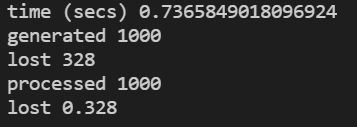
\includegraphics[scale=0.9]{source/2}}
		\centering\caption{1000 заявок}
	\end{figure}
	
	\begin{figure}[h!]
		\centering{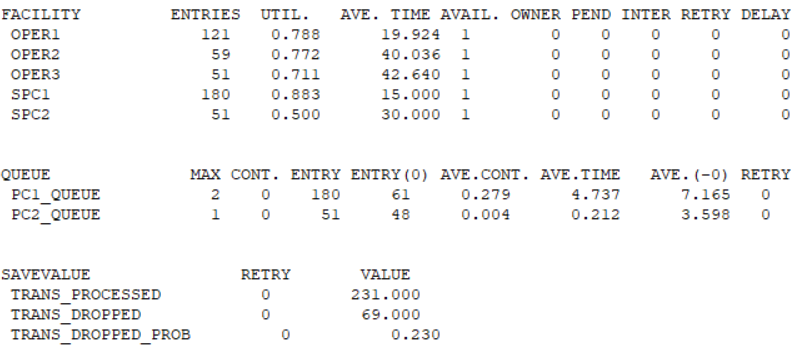
\includegraphics[scale=0.9]{source/3}}
		\centering\caption{3000 заявок}
	\end{figure}
	
	\section*{Вывод}
	\addcontentsline{toc}{section}{Вывод}
	Основываясь на примерах работы системы при 300, 1000 и 3000 посетителях, можно сделать вывод, что процент потерь 
	примерно равен 33\%. Это значит, что следует сделать аттракционы менее страшными, чтобы избежать потерь.
	
	
	\clearpage
	\section*{Листинги}
	\addcontentsline{toc}{section}{Листинги}
	
	\begin{lstlisting}[caption=main.py]
		from time import time
		from UniformDistribution import UniformDistribution
		from Generator import Generator
		from Operator import Operator
		from Attraction import Attraction
		
		timeStep = 0.01
		
		
		def DoStep(generator, operators, Attractions, visitorInfo, newGenerate=True):
			if newGenerate:
				res = generator.UpdateTime(timeStep)
				if res:       
					visitorInfo['generated'] += 1
			
			for curOperator in operators:
				curOperator.UpdateTime(timeStep)
			
			for curAttraction in Attractions:
				res = curAttraction.UpdateTime(timeStep)
				if res == 0:
					visitorInfo['processed'] += 1
				elif res == -1:
					visitorInfo['lost'] += 1
		
		def modeling(generator, operators, Attractions, incomingVisitorAmount):
			visitorInfo = {'generated': 0, 'lost': 0, 'processed': 0}
			
			while visitorInfo['generated'] < incomingVisitorAmount:
				DoStep(generator, operators, Attractions, visitorInfo)
			
			while visitorInfo['processed'] < incomingVisitorAmount:
				DoStep(generator, operators, Attractions, visitorInfo, False)
			
			return visitorInfo
		
		
		def main():
			firstQueueGroup = [[], [], []]
			secondQueueGroup = [[], []]
			
			clientGenerator = Generator(UniformDistribution(1, 5), firstQueueGroup)
			
			operators = [
				Operator(firstQueueGroup[0], secondQueueGroup, UniformDistribution(2, 5)),    
				Operator(firstQueueGroup[1], secondQueueGroup, UniformDistribution(4, 8)),
				Operator(firstQueueGroup[2], secondQueueGroup, UniformDistribution(10, 15))    
			]
			
			Attractions = [
				Attraction(secondQueueGroup[0], UniformDistribution(5, 9)),   
				Attraction(secondQueueGroup[1], UniformDistribution(10, 25))   
			]
			
			totalVisitors = 300
			
			tStart = time()
			res = modeling(clientGenerator, operators, Attractions, totalVisitors)
			
			print('time (secs)', time() - tStart)
			for key in res.keys():
				print(key, res[key])
			
			print('lost', res['lost'] / totalVisitors)
			
		
		if __name__ == '__main__':
			main()		
	\end{lstlisting}

	\begin{lstlisting}[caption=Generator.py]
	class Generator:
		def __init__(self, distribution):
			self.timeDistribution = distribution
			self.queues = queueGroup
			self.finishTime = 0
			self.visitorId = -1
		
		def UpdateTime(self, dt):
			self.finishTime -= dt
		
			if self.finishTime <= 1e-5:
				self.finishTime = self.timeDistribution.generate()
				self.visitorId += 1
				self.AddToQueue()
				return True
		
			return False
		
		def AddToQueue(self):
			minLen = len(self.queues[0])
			minQueueIndex = 0
			for i in range(1, len(self.queues)):
				if len(self.queues[i]) < minLen:
					minLen = len(self.queues[i])
					minQueueIndex = i
			self.queues[minQueueIndex].append(self.visitorId)	
	\end{lstlisting}
	
	\begin{lstlisting}[caption=Attraction.py]
		class Attraction:
			def __init__(self, visitorsQueue, distribution):
				self.timeDistribution = distribution
				self.busy = False
				self.visitorsQueue = visitorsQueue
				self.finishTime = 0
		
			def UpdateTime(self, dt):
				self.finishTime -= dt
				if self.busy and self.finishTime <= 1e-5:
					self.busy = False
					return 0
				
				if not self.busy and len(self.visitorsQueue) != 0:
					if random() < 0.75:
					self.visitorsQueue.pop(0)
					self.finishTime = self.timeDistribution.generate()
					self.busy = True
					return 1
				else:
					return -1
				
				return 2
	\end{lstlisting}	

	\begin{lstlisting}[caption=Operator.py]
	class Operator:
		def __init__(self, queue, queueGroup, distribution):
			self.timeDistribution = distribution
			self.busy = False
			self.queue = queue
			self.queues = queueGroup
			self.curVisitor = None
			self.finishTime = 0
		
		def acceptVisitor(self):
			self.busy = True
			self.curVisitor = self.queue.pop(0)
			self.finishTime = self.timeDistribution.generate()
		
		def finishCurVisitor(self):
			self.AddToQueue()
			self.busy = False
			self.curVisitor = None
		
		def AddToQueue(self):
		minLen = len(self.queues[0])
			minQueueIndex = 0
			for i in range(1, len(self.queues)):
				if len(self.queues[i]) < minLen:
					minLen = len(self.queues[i])
					minQueueIndex = i
			self.queues[minQueueIndex].append(self.curVisitor)
		
		def UpdateTime(self, dt):
			self.finishTime -= dt
			if not self.busy and len(self.queue) > 0:
				self.acceptVisitor()
		
			if self.busy and self.finishTime <= 1e-5:
				self.finishCurVisitor()
				return 0
		return 2	
	\end{lstlisting}
\end{document}